\section{System Architecture and Current Methods}

Figure~\ref{fig:pipeline-overview} summarizes the current AGAI pipeline. Solid arrows represent the deployed runtime path. Dashed arrows represent the offline stage-2 data-generation path used for the current dual-report pilot.

\begin{figure*}[t]
\centering
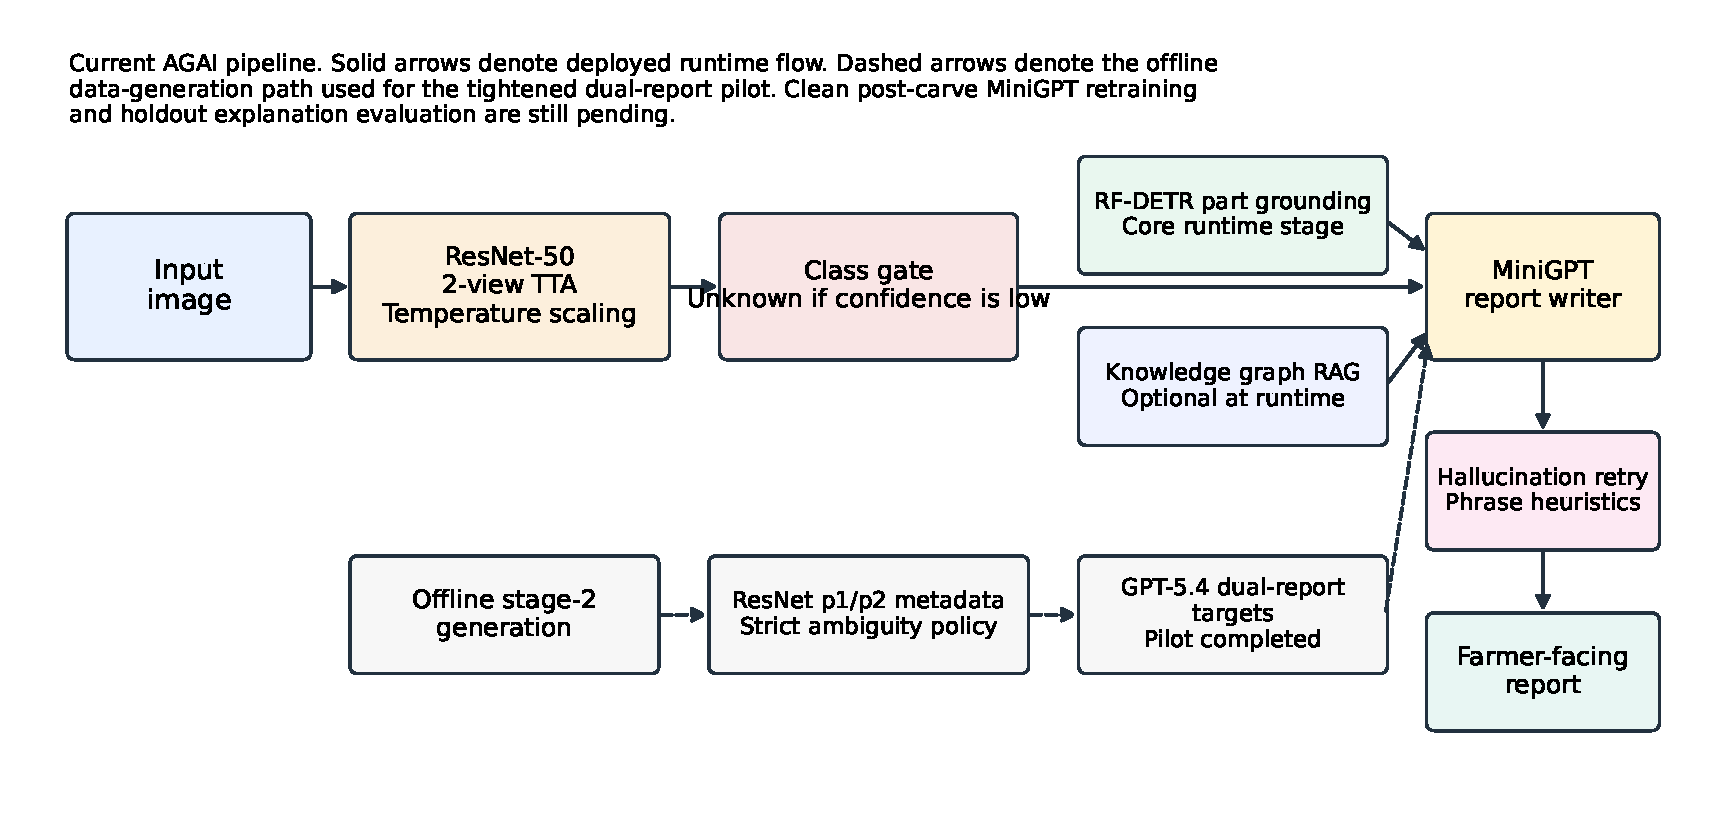
\includegraphics[width=\textwidth]{figures/generated/pipeline_overview.pdf}
\caption{Current AGAI pipeline. The classifier and runtime prompt assembly are deployed. The dual-report path is currently an offline pilot for stage-2 regeneration. Clean MiniGPT retraining and clean holdout explanation evaluation are still pending.}
\label{fig:pipeline-overview}
\end{figure*}

\subsection{Classifier Backbone, Test-Time Augmentation, and Calibration}

The active classifier is a ResNet-50 \citep{he2016resnet}. The repository training script uses standard ImageNet normalization, moderate geometric and photometric augmentation during training, and a 256-pixel evaluation crop. At inference time, the deployed classifier averages two views: the original center-cropped image and its horizontal flip. If the raw logit vector for image $x$ is $z(x) \in \mathbb{R}^{7}$ and the learned temperature is $T > 0$, then the deployed class distribution is
\begin{equation}
\bar{p}(c \mid x)
= \frac{1}{2}\left[
\mathrm{softmax}\!\left(\frac{z(x)}{T}\right)_c
+
\mathrm{softmax}\!\left(\frac{z(\mathrm{flip}(x))}{T}\right)_c
\right].
\label{eq:tta-calibration}
\end{equation}

The predicted class is the maximum-probability class under $\bar{p}(c \mid x)$:
\begin{equation}
\hat{y}(x) = \arg\max_{c \in \mathcal{C}} \bar{p}(c \mid x),
\end{equation}
where $\mathcal{C}$ is the seven-class label set.

The current balanced-split checkpoint uses a learned temperature of 0.7810 on the active holdout evaluation. The deployed classifier continues to use the same two-view TTA policy.

\subsection{Runtime Acceptance Gate}

The runtime application does not accept every classifier output as an actionable diagnosis. It applies a per-class threshold gate:
\begin{equation}
\mathrm{accept}(x)
= \mathbf{1}\!\left[\bar{p}(\hat{y}(x)\mid x) \ge \tau_{\hat{y}(x)}\right].
\label{eq:threshold-gate}
\end{equation}

The current thresholds are
\begin{align}
\tau_{\mathrm{healthy}} &= 0.40, &
\tau_{\mathrm{overwatered}} &= 0.60, &
\tau_{\mathrm{root\ rot}} &= 0.65, \nonumber \\
\tau_{\mathrm{drought}} &= 0.65, &
\tau_{\mathrm{frost}} &= 0.70, &
\tau_{\mathrm{gray\ mold}} &= 0.60, \quad
\tau_{\mathrm{white\ mold}} = 0.60.
\label{eq:class-thresholds}
\end{align}
The default threshold for any unmapped class is 0.55. A second conservative guard in the runtime code demotes the prediction to \texttt{unknown} when the accepted top-1 probability falls below 0.50 after prompt assembly.

The system also logs $p_1$, $p_2$, and the margin $p_1-p_2$ for later analysis. A margin threshold of 0.08 exists in the codebase only as a logging quantity. It is not currently applied at runtime. This is important because the current classifier claims in this paper are threshold-only runtime claims, not threshold-plus-margin claims.

\subsection{Grounded Runtime Report Path}

The report-generation stage is deliberately downstream of the classifier. The ResNet label is injected into the prompt as the authoritative diagnosis, RF-DETR contributes the visible-part and not-visible-part evidence summary, and the report writer is expected to explain that grounded diagnosis rather than re-predict it.

The runtime stack has one required grounding stage and two additional support mechanisms:
\begin{enumerate}[leftmargin=1.3em]
\item \textbf{RF-DETR part grounding.} The detector is part of the runtime pipeline. Its part detections are converted into visible-part and not-visible-part lists that constrain what the report is allowed to claim about the image.
\item \textbf{Knowledge-graph retrieval.} If the local disease QA resources load successfully, retrieved snippets can be appended to the report prompt as supplemental context.
\item \textbf{Heuristic hallucination retry.} A phrase-triggered retry gate attempts to catch certain known overclaims by matching hard-coded substrings such as disease names or visual claims. This is currently heuristic and not yet calibrated against a clean false-positive budget.
\end{enumerate}

All three components operate locally at runtime. GPT is not used at inference time.

\subsection{Current MiniGPT Configuration}

The current MiniGPT training configuration uses a MiniGPT-v2 architecture \citep{chen2023minigptv2} with a Llama 2 chat backbone \citep{touvron2023llama2} and LoRA adaptation \citep{hu2021lora}. The active settings specify a 448-pixel image size, maximum text length 500, LoRA rank 64, LoRA alpha 128, dropout 0.05, batch size 2 per GPU, 8 gradient accumulation steps, and 20 epochs with a 10\% auto-validation split. These are the active training settings in the repository, not proof that a clean MiniGPT retrain on the newly balanced stage-2 dataset has already been completed.

\subsection{Offline Dual-Report Generation Policy}

The current stage-2 redesign uses GPT-5.4 only offline. Every image receives one standard farmer-facing report. Some images also receive a second report, but only under a deliberately strict ambiguity policy.

Let the ground-truth folder label be $g(x)$, the top-1 classifier label be $y_1(x)$, and the top-2 classifier label be $y_2(x)$. The strongest competing class used for the offline policy is
\begin{equation}
a(x) =
\begin{cases}
y_2(x), & y_1(x) = g(x), \\
y_1(x), & y_1(x) \neq g(x).
\end{cases}
\label{eq:alt-class}
\end{equation}

The second report is allowed to be ambiguity-aware only when the candidate pair is semantically plausible and the probabilities are genuinely close. The current allowed pair set is
\begin{equation}
\mathcal{A} =
\left\{
\begin{aligned}
&\{\mathrm{gray\ mold}, \mathrm{white\ mold}\}, \\
&\{\mathrm{drought}, \mathrm{overwatered}\}, \\
&\{\mathrm{drought}, \mathrm{frost}\}, \\
&\{\mathrm{healthy}, \mathrm{overwatered}\}, \\
&\{\mathrm{root\ rot}, \mathrm{overwatered}\}
\end{aligned}
\right\}.
\label{eq:allowed-pairs}
\end{equation}

Under the current builder, a second report is marked \emph{ambiguous} only if one of two cases holds:
\begin{align}
y_1(x) = g(x), \qquad
\bar{p}(y_1 \mid x) - \bar{p}(y_2 \mid x) &\le 0.10, \nonumber \\
\bar{p}(y_2 \mid x) \ge 0.15, \qquad
\{g(x), y_2(x)\} &\in \mathcal{A}, \label{eq:amb-case-1} \\
y_1(x) \neq g(x), \qquad
\mathrm{rank}(g(x)) = 2, \nonumber \\
\bar{p}(y_1 \mid x) - \bar{p}(g \mid x) &\le 0.10, \nonumber \\
\bar{p}(g \mid x) \ge 0.15, \qquad
\{g(x), y_1(x)\} &\in \mathcal{A}. \label{eq:amb-case-2}
\end{align}

If the classifier is correct and the margin is clear, the second report becomes a \emph{standard variant} rather than an ambiguity report. If the classifier is wrong and the ground truth is not a close rank-2 competitor, the second report is skipped entirely. This prevents obvious classifier failures from being laundered into fake ambiguity.

This policy is currently a pilot-stage data-generation policy only. It is not yet a claim about the live runtime behavior of the deployed report generator.
